\begin{figure}[htbp]
\centering
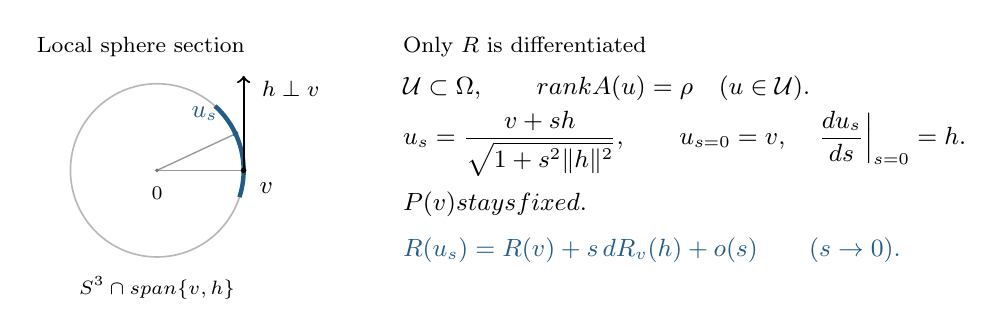
\begin{tikzpicture}[x=1cm,y=1cm,font=\small]
  \definecolor{tangentblue}{RGB}{35,92,135}

  \node[anchor=west,font=\footnotesize] at (0,3.02)
    {Local sphere section};
  \coordinate (O) at (1.65,1.45);
  \coordinate (V) at (2.75,1.45);
  \coordinate (Us) at (2.6469,1.9149); %
  \draw[black!28,line width=0.6pt] (O) circle[radius=1.1];

  \draw[tangentblue,line width=1.6pt]
    (2.6962,1.1101) arc[start angle=-18,end angle=48,radius=1.1];
  \draw[black!40,line width=0.5pt] (O) -- (V);
  \draw[black!40,line width=0.5pt] (O) -- (Us);
  \fill[black!55] (O) circle[radius=0.025];
  \node[anchor=north,font=\scriptsize] at (1.65,1.36) {$0$};

  \draw[->,line width=0.8pt] (V) -- (2.75,2.65);
  \node[anchor=west,font=\footnotesize] at (2.86,2.49) {$h\perp v$};
  \fill (V) circle[radius=0.035];
  \node[anchor=north west] at (2.83,1.42) {$v$};
  \fill[tangentblue] (Us) circle[radius=0.037];
  \node[anchor=south east,text=tangentblue] at (2.54,1.96) {$u_s$};
  \node[anchor=north,font=\scriptsize] at (1.65,0.22)
    {$S^3\cap\operatorname{span}\{v,h\}$};

  \node[anchor=west,font=\footnotesize] at (4.65,3.02)
    {Only $R$ is differentiated};
  \node[anchor=west] at (4.65,2.49)
    {$\mathcal U\subset\Omega,\qquad \operatorname{rank}A(u)=\rho\quad(u\in\mathcal U).$};
  \node[anchor=west] at (4.65,1.79)
    {$\displaystyle u_s=\frac{v+sh}{\sqrt{1+s^2\|h\|^2}},
      \qquad u_{s=0}=v,\quad \left.\frac{du_s}{ds}\right|_{s=0}=h.$};
  \node[anchor=west] at (4.65,1.02)
    {$P(v)\text{ stays fixed.}$};
  \node[anchor=west,text=tangentblue] at (4.65,0.43)
    {$R(u_s)=R(v)+s\,dR_v(h)+o(s)\qquad(s\to0).$};
\end{tikzpicture}
\caption{A schematic local tangent step, for a fixed nonzero $h\in v^\perp$.
The highlighted arc lies in a chosen constant-rank neighborhood $\mathcal U$;
the expansion of $R$ is used only for small $s$ with $u_s\in\mathcal U$.
The pictured section belongs to the parameter sphere, whereas $P(v)$
and $R(u_s)$ act on the separate block spaces $\mathbb R^a$ and
$\mathbb R^c$.}
\label{fig:local-tangent}
\end{figure}
